% !TEX root = thesis.tex
\chapter{Implementation}
\label{sec:implementation}

This chapter describes the realization of the architecture developed in Chapter \ref{sec:design_methodology} as a synthesizable and board-deployable system. The proposed \gls{sdsp} learning path is integrated with the generated Spiker+ accelerator, while the surrounding system provides the control, data-transfer, and memory-access mechanisms required to operate the accelerator on an embedded \gls{fpga} platform. The implementation therefore covers both the modified neural-network hardware and its connection to the processor-side software environment.

The chapter first introduces the target platform and the PYNQ overlay abstraction. The subsequent sections describe the realization of the learning-related \gls{rtl} modules, their integration into the Spiker+ hierarchy, and the board-level communication path used to transfer spike data and control the accelerator. Verification and implementation results are presented separately in Chapter \ref{sec:results_and_evaluation}.

\section{Target Platform and PYNQ Overlay}
\label{subsec:target-platform-and-overlay}

The implementation targets the Digilent PYNQ-Z1 development board. The board combines an embedded processor and reconfigurable logic in a single Zynq-7000 device and is supported by the PYNQ software environment. This combination is suitable for the present work because processor-side preparation and control can be separated from the latency-sensitive spike processing and online weight updates implemented in hardware.

\subsection{PYNQ-Z1 Hardware Platform}

Figure \ref{fig:pynq-z1-board} shows the PYNQ-Z1 board used for deployment. Its central device is the XC7Z020-1CLG400C Zynq-7000 All Programmable \gls{soc}. The device consists of a \gls{ps}, containing a dual-core ARM Cortex-A9 processor and the fixed memory and peripheral controllers, and a \gls{pl}, which contains the configurable logic resources used for the \gls{snn} accelerator \cite{DigilentPYNQZ1Manual}.

\begin{figure}[t]
	\centering
	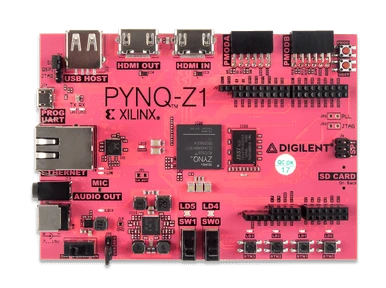
\includegraphics[width=0.78\linewidth]{figures/pynq_z1_board_official.png}
	\caption{Digilent PYNQ-Z1 Development Board \cite{DigilentPYNQZ1Product}}
	\label{fig:pynq-z1-board}
\end{figure}

Table \ref{tab:pynq-z1-resources} summarizes the platform resources most relevant to this implementation. The 512~MB external \gls{ddr} \gls{sdram} provides storage for input spike sequences and processor-side data, while the configurable logic implements the accelerator and its interface logic. The available logic slices and \gls{bram} resources are particularly relevant to the parallel neuron datapaths and writable synaptic-weight memories. Although the board also provides video, audio, Ethernet, USB, Pmod, and Arduino-compatible interfaces, these peripherals are not required by the implemented accelerator and are therefore not considered further.

\begin{table}[htbp]
	\centering
	\caption{PYNQ-Z1 Resources Relevant to the Implemented System \cite{DigilentPYNQZ1Manual}}
	\label{tab:pynq-z1-resources}
	\begin{tabularx}{0.92\linewidth}{@{}lX@{}}
		\toprule
		\textbf{Resource} & \textbf{Platform characteristic} \\
		\midrule
		Zynq device & XC7Z020-1CLG400C \\
		Processing system & Dual-core ARM Cortex-A9, up to 650\,MHz \\
		Programmable logic & 13,300 logic slices and 220 DSP slices \\
		On-chip memory & 630~KB of block RAM \\
		External memory & 512~MB DDR3 with a 16-bit data bus \\
		Boot and storage & 16~MB QSPI flash and microSD interface \\
		\bottomrule
	\end{tabularx}
\end{table}

The functional relationship between the two parts of the Zynq device is illustrated in Figure \ref{fig:pynq-overlay-concept}. The \gls{ps} executes the PYNQ software stack and accesses the external DDR memory, whereas custom peripherals and accelerators are instantiated in the \gls{pl}. Standard AXI connections provide control and data exchange between the two domains. In the implemented system, a general-purpose AXI master port is used for accelerator control, a high-performance AXI slave port gives the \gls{dma} engine access to DDR, and a 100\,MHz fabric clock drives the accelerator and its interface logic. Completion and error events can be returned to the processor through fabric interrupts.

\begin{figure}[t]
	\centering
	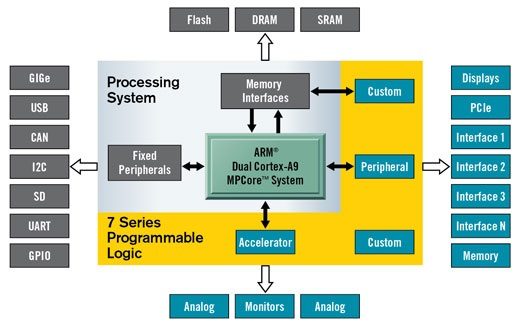
\includegraphics[width=0.78\linewidth]{figures/pynq_overlay_concept_official.png}
	\caption{Processing-System and Programmable-Logic Organization of the Zynq-7000 \gls{soc} \cite{PYNQOverlays}}
	\label{fig:pynq-overlay-concept}
\end{figure}

This heterogeneous organization assigns tasks according to their computational characteristics. The processor handles configuration, memory management, and test coordination, while the \gls{pl} performs deterministic spike processing and local synaptic updates. The external DDR memory is therefore used as the exchange point for input data rather than as storage for individual synaptic updates; the latter remain inside the accelerator's writable weight memories.

\subsection{PYNQ Overlay Abstraction}

PYNQ represents a hardware design as an \emph{overlay}: a configurable hardware system that can be loaded into the \gls{pl} and controlled from Python running on the \gls{ps}. A typical overlay is distributed with a bitstream file (\texttt{.bit}) and a hardware handoff file (\texttt{.hwh}). The bitstream configures the programmable logic, while the hardware description provides the address map, instantiated \gls{ip} blocks, clocks, and interrupt connections required by the PYNQ software interface \cite{PYNQOverlayLoading,PYNQOverlayDesign}.

For this work, the overlay forms the deployment container around the Spiker+-\gls{sdsp} accelerator. It includes the Zynq processing system, the DDR-facing \gls{dma} path, the AXI control interconnect, buffering for the input stream, and the accelerator wrapper. From the processor side, the software loads the overlay, allocates the input buffers in DDR, configures the accelerator through memory-mapped control registers, starts the data transfer, and reads the produced status and classification results. The learning computation itself remains entirely in the \gls{pl}; the Python environment is used to operate and evaluate the hardware rather than to calculate weight updates.

Loading the overlay configures the complete \gls{pl} design. In this thesis, it is not used to exchange learning modules during execution and should therefore not be confused with the \gls{dpr} approach discussed in Section \ref{subsec:dpr-applicability}. The overlay provides a convenient software-visible boundary for the statically implemented system, whereas the internal \gls{snn} and \gls{sdsp} architecture remains fixed for the duration of an experiment.

\section{RTL Architecture and Module Hierarchy}
\label{subsec:rtl-architecture}

The final Vivado implementation is organized in three nested levels. The generated top-level wrapper contains the complete block design, the block design instantiates the packaged SNN--SDSP accelerator as a custom \gls{ip} core, and the custom IP contains the AXI wrapper together with the complete Spiker+ network and learning hierarchy. This organization keeps the board-specific processing-system and data-movement infrastructure outside the reusable accelerator IP while allowing the complete design to be synthesized through one generated top-level entity. Figure \ref{fig:rtl-hierarchy} shows this final elaborated hierarchy.

\begin{figure}[t]
	\centering
	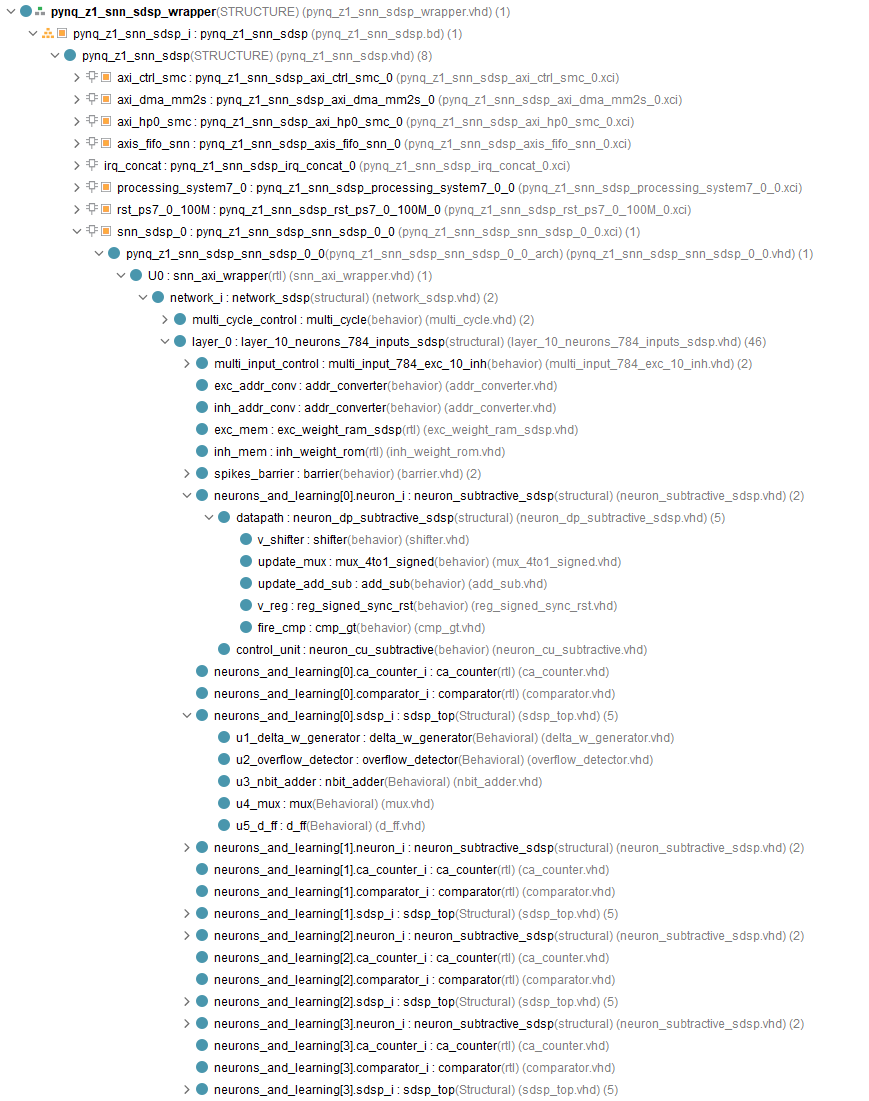
\includegraphics[width=0.92\linewidth]{figures/rtl_hierarchy.png}
	\caption{Final Elaborated \gls{rtl} Hierarchy of the PYNQ-Z1 \gls{snn}--\gls{sdsp} System}
	\label{fig:rtl-hierarchy}
\end{figure}

At the root of the hierarchy, the Vivado-generated entity \texttt{pynq\_z1\_snn\_sdsp\_wrapper} instantiates the block design as \texttt{pynq\_z1\_snn\_sdsp\_i}. Only the DDR and fixed \gls{ps} pins are exposed at this level. The expanded block-design hierarchy contains the Zynq processing system, reset generator, two AXI SmartConnect instances, the memory-to-stream \gls{dma}, the AXI4-Stream FIFO, the interrupt concatenation block, and the custom accelerator instance \texttt{snn\_sdsp\_0}. The accelerator is therefore part of the block design rather than a separate entity instantiated beside it at the project root.

The generated shell of \texttt{snn\_sdsp\_0} instantiates \texttt{snn\_axi\_wrapper} as \texttt{U0}. This module is the top level of the handwritten accelerator logic and contains \texttt{network\_sdsp} as \texttt{network\_i}. Below it, the hierarchy follows the original Spiker+ organization through the multi-cycle controller, the modified output layer, and the generated neuron lanes. The first lane is expanded in Figure \ref{fig:rtl-hierarchy} to expose its neuron datapath, calcium counter, comparator, and \texttt{sdsp\_top} instance. The same generated structure is repeated for all ten output neurons.

\subsection{Top-Level Organization}

The block design supplies the accelerator IP with the 100\,MHz \gls{pl} clock generated by the processing system and the active-low peripheral reset generated by \texttt{rst\_ps7\_0\_100M}. The AXI \gls{dma} reads packed spike data from DDR through the high-performance memory path. Its 32-bit MM2S output passes through \texttt{axis\_fifo\_snn} before reaching the AXI4-Stream slave interface of \texttt{snn\_sdsp\_0}. The processing-system AXI master reaches both the DMA control interface and the accelerator's AXI4-Lite register interface through \texttt{axi\_ctrl\_smc}. The DMA and accelerator interrupt outputs are combined by \texttt{irq\_concat} and returned to the \gls{ps}. These infrastructure blocks are visible in the upper part of Figure \ref{fig:rtl-hierarchy}; their connections are discussed in detail in Section \ref{subsec:block-design-integration}.

Inside the packaged IP, the AXI4-Stream and AXI4-Lite ports terminate directly at \texttt{snn\_axi\_wrapper}. The wrapper, \texttt{network\_sdsp}, the learning logic, and the synaptic memories all use the same 100\,MHz fabric clock. No clock-domain crossing is therefore required within the accelerator hierarchy. Packaging the entire hierarchy below \texttt{snn\_axi\_wrapper} also ensures that the block design interacts only with standard AXI, clock, reset, and interrupt interfaces; no internal neuron or learning signal crosses the IP boundary.

The reset structure distinguishes between the platform reset and an accelerator soft reset. The active-low platform reset initializes the complete AXI wrapper and network. A software-generated soft-reset pulse is combined with the platform reset before entering \texttt{network\_sdsp}. This permits the neural state and transaction counters to be restarted without reloading the overlay. Runtime settings, including the learning and teacher controls and the periodic-event intervals, remain in the AXI register bank until they are explicitly changed or the platform reset is asserted.

Within \texttt{snn\_axi\_wrapper}, the \texttt{network\_sdsp} entity contains a multi-cycle controller and one modified Spiker+ layer. The layer contains the generated multi-input controller, the excitatory and inhibitory address converters, the two weight memories, the output barrier, and ten parallel neuron-and-learning lanes. Each lane consists of a modified \gls{lif} neuron, a calcium counter, a condition comparator, and an \texttt{sdsp\_top} weight-update unit. The hierarchy view expands the internal modules of lane zero and lists the repeated instances of the following lanes, confirming that the neuron and learning logic are generated together beneath the modified layer.

\subsection{AXI Wrapper and Input Buffering}

The \texttt{snn\_axi\_wrapper} converts the board-level AXI transactions into the vector and handshake interfaces required by \texttt{network\_sdsp}. Its implemented data and control paths are summarized in Figure \ref{fig:snn-axi-wrapper-rtl}. The AXI4-Stream path carries input spikes, whereas AXI4-Lite provides configuration, status, and result access.

\begin{figure}[t]
	\centering
	\makebox[\linewidth][c]{%
		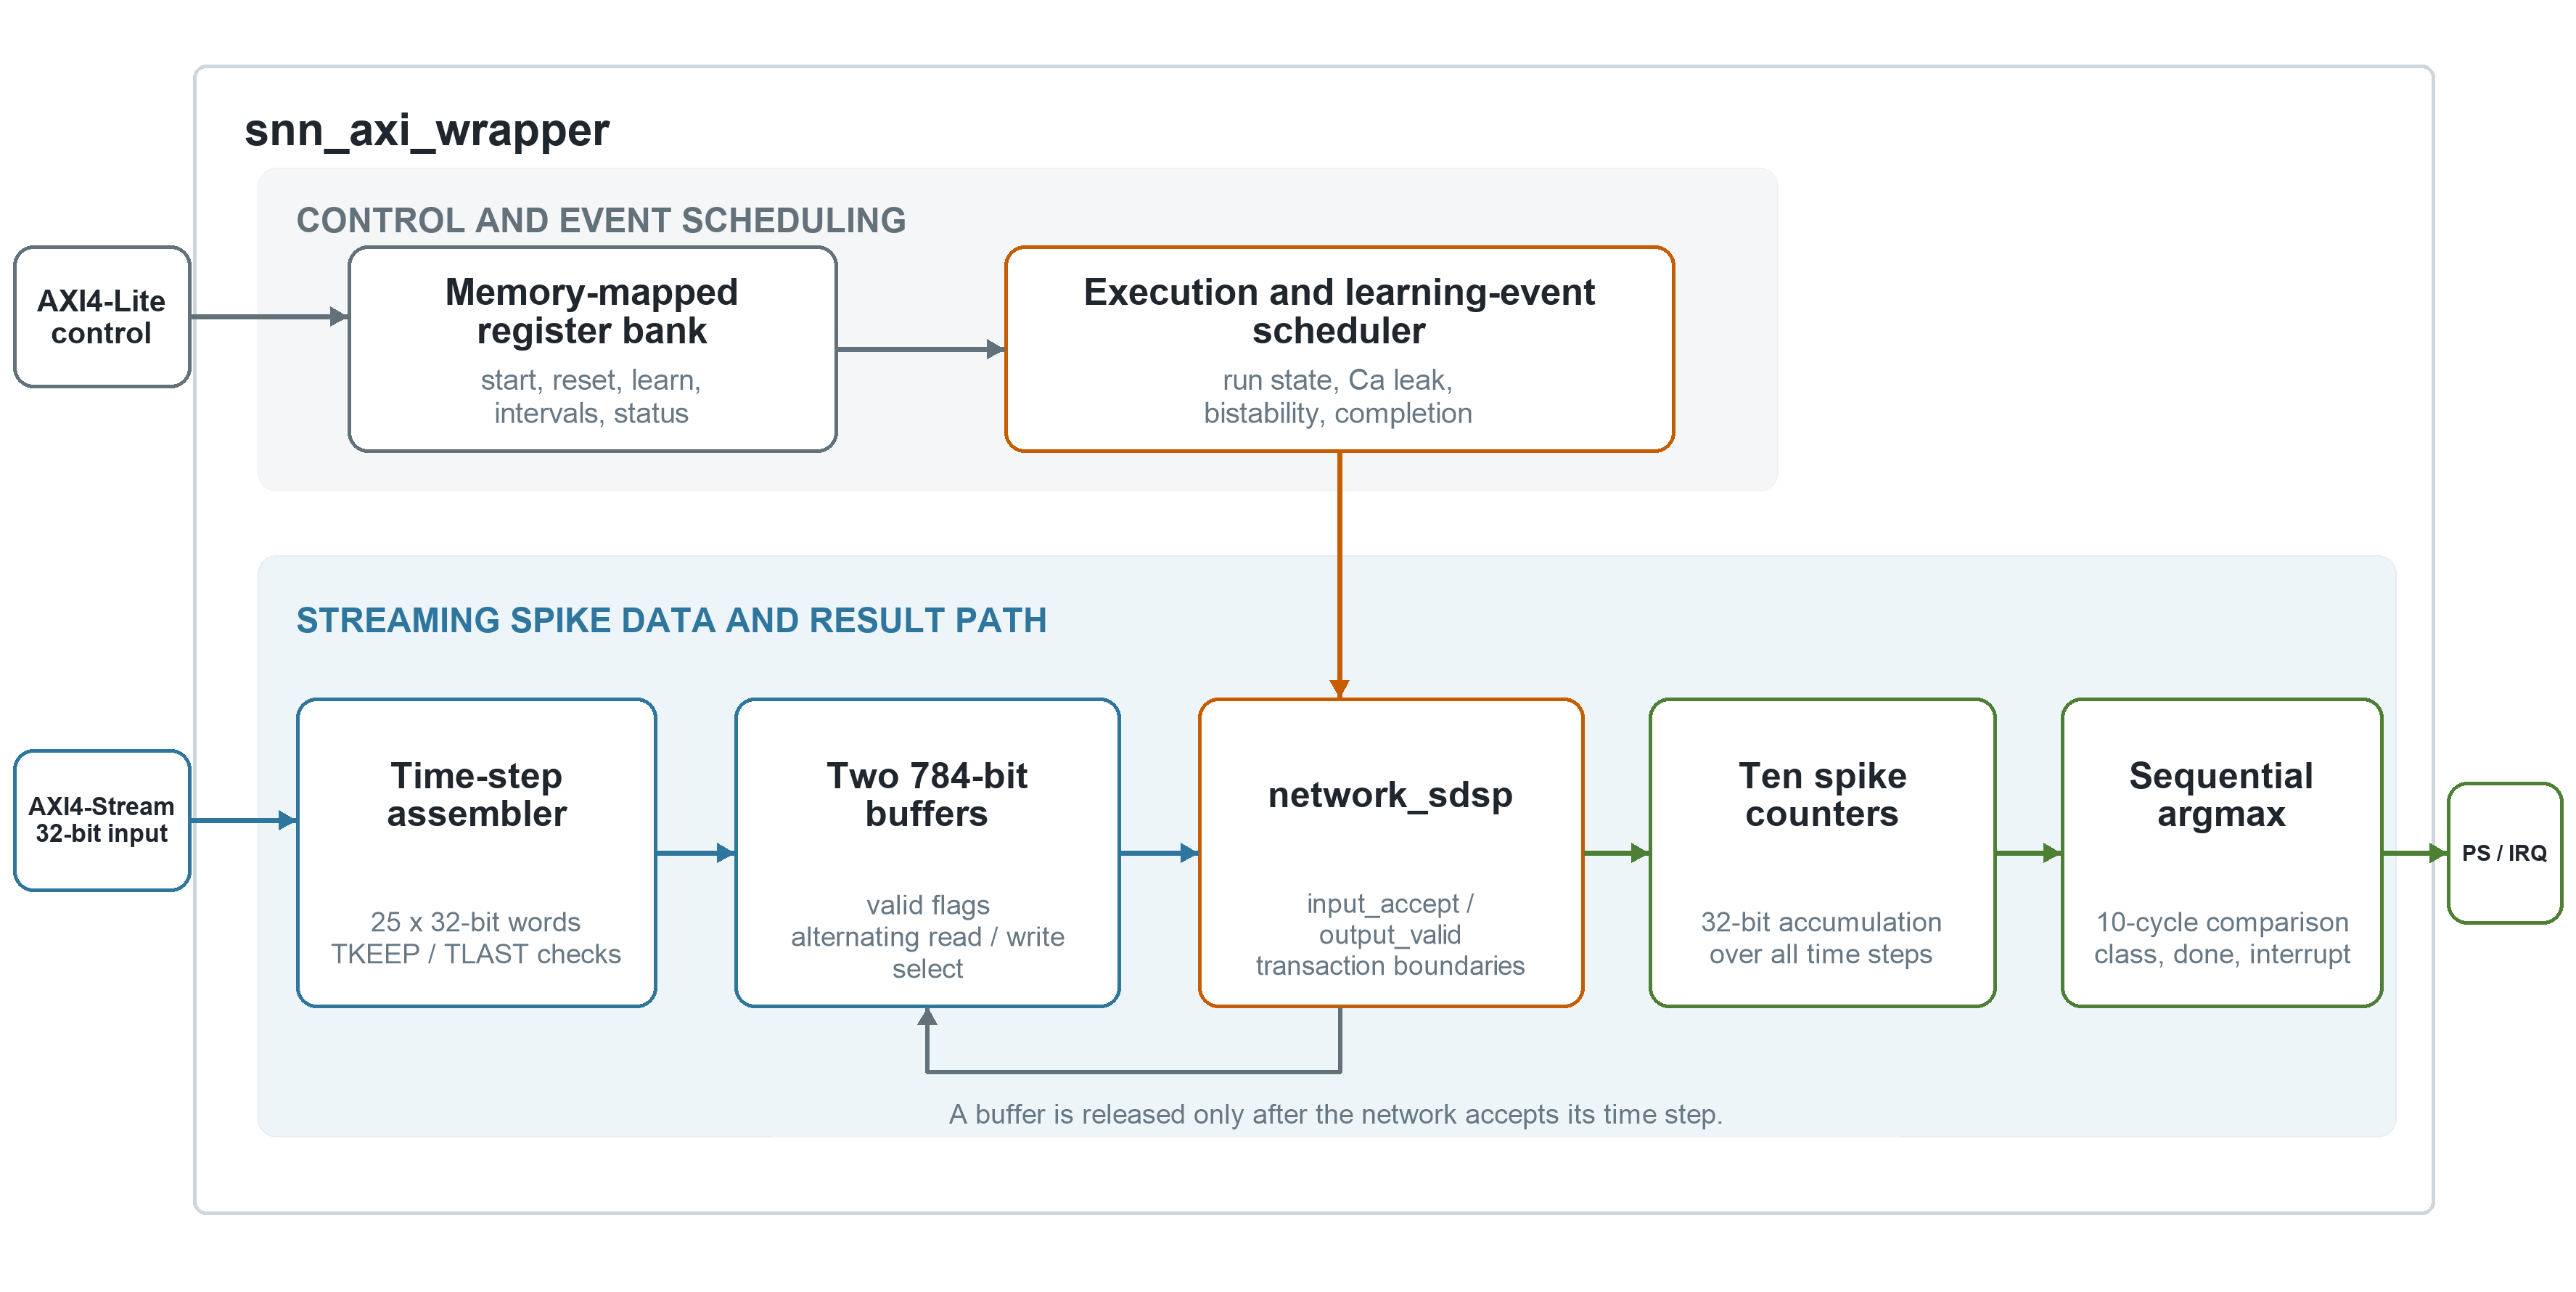
\includegraphics[width=1.10\linewidth]{figures/snn_axi_wrapper_rtl.png}%
	}
	\caption{Implemented Data and Control Flow within \texttt{snn\_axi\_wrapper}}
	\label{fig:snn-axi-wrapper-rtl}
\end{figure}

One network time step contains 784 binary input spikes. The wrapper reconstructs this vector from 25 consecutive 32-bit AXI4-Stream words. Words 0 to 23 contain spike bits 0 to 767, and the lower 16 bits of the final word contain spike bits 768 to 783, while its upper 16 bits serve as padding. The implementation checks \texttt{TKEEP} for every accepted word and expects \texttt{TLAST} only on the final word of the complete input sequence. Unexpected byte enables or an incorrectly positioned \texttt{TLAST} set sticky error flags that can be inspected through the control interface.

Two 784-bit registers form a ping-pong input buffer. The streaming interface assembles a new time step in the buffer selected by \texttt{write\_select}, while the network reads the buffer selected by \texttt{read\_select}. A valid bit is maintained for each buffer. Stream readiness is asserted only when the selected write buffer is empty and the configured number of time steps has not yet been received. Similarly, \texttt{sample\_ready} is presented to the network only when the selected read buffer contains a complete vector. When the network asserts \texttt{input\_accept}, the corresponding valid flag is cleared and the read selection is toggled. Input transfer and network processing can consequently overlap without allowing a partially assembled vector to reach the \gls{snn}.

The AXI4-Lite register bank stores the runtime controls and returns the accelerator status. A start command is retained as \texttt{start\_pending} until both the network and the first input buffer are ready. Dedicated registers hold the learning, teacher, bistability, and interrupt enables, together with the teacher label and current and the calcium-leak and bistability intervals. Countdown registers generate the periodic learning events, avoiding division or modulo operations in the synthesized datapath. A calcium-leak event is issued as a single-cycle pulse, whereas a bistability event remains active for the complete synapse scan so that all excitatory addresses can be examined.

For every valid network output, ten 32-bit counters accumulate the spikes produced by the output neurons. After the final time step has completed, the wrapper determines the output class through a sequential argmax scan. One counter is compared per clock cycle, replacing a long combinational chain of nine comparisons. When the tenth counter has been examined, the wrapper stores the selected class, clears the active state, sets a sticky completion flag, and asserts the interrupt if it has been enabled.

\subsection{Network, Layer, and Neuron RTL}

The \texttt{network\_sdsp} entity preserves the multi-cycle execution model of the generated Spiker+ design. In the implemented configuration, one run contains 100 time steps. The multi-cycle controller requests the next sample only when the modified layer reports that it is ready, and the additional \texttt{sample\_ready} input prevents it from advancing before the AXI wrapper has assembled a complete spike vector. The signals \texttt{input\_accept} and \texttt{out\_spikes\_valid} expose the exact clock cycles at which the input buffer can be released and the corresponding output can be counted.

The layer contains 784 excitatory inputs and ten output neurons. The ten output spikes are also returned as inhibitory inputs, retaining the recurrent competition of the generated network. The multi-input controller scans the excitatory addresses first and subsequently processes the ten inhibitory inputs. For a selected presynaptic address, one 30-bit memory word supplies one three-bit weight to each of the ten neurons. The presynaptic inputs are therefore processed sequentially, while all postsynaptic neurons operate in parallel.

The neuron controller retains the original initialization, excitatory integration, inhibitory integration, leakage, firing, and subtractive-reset operations. Its datapath stores the membrane potential as a 16-bit signed value and exposes this register to the learning comparator. Excitatory weights are represented as unsigned values and are zero-extended before they enter the membrane-potential adder. Inhibitory weights retain their signed representation and are sign-extended. This distinction is required because an excitatory three-bit code with its most significant bit set must remain a positive magnitude rather than being interpreted as a negative two's-complement number.

The neuron-ready signals are combined with the output-barrier status to form the layer-ready condition. The barrier captures the ten output spikes at the end of a time step and retains them for the recurrent inhibitory path. Additional registers record when a step has been accepted and produce a one-cycle \texttt{step\_valid} pulse only after all neuron operations and the barrier transaction have completed. These signals provide the precise transaction boundaries used by the AXI wrapper.

\subsection{Learning Lanes and Synaptic Memory}

The learning hardware is instantiated with a VHDL \texttt{for-generate} statement, producing one learning lane for each output neuron. A lane contains the neuron state, a 3-bit saturating calcium counter, the \gls{sdsp} condition comparator, and the registered weight update datapath. The calcium counter is cleared at the beginning of a new sample, increments on a postsynaptic spike, and decrements on a calcium-leak event. If a spike and a leak event occur in the same clock cycle, the stored value is retained. The comparator treats the calcium value as unsigned and the membrane potential as a signed two's-complement quantity when generating the \texttt{up} and \texttt{down} conditions.

The ten \texttt{sdsp\_top} instances receive the current 30-bit excitatory word as ten independent three-bit fields. Each instance evaluates its local conditions and registers a candidate next weight. The update enable is generated from the global learning enable, the delayed excitatory phase, the validity of the current address, and the presence of either a presynaptic spike or a bistability event. When learning is disabled, the update registers do not alter the stored synaptic state.

Excitatory weights are stored in \texttt{exc\_weight\_ram\_sdsp}, a 784-by-30-bit simple-dual-port memory. Each word contains the ten three-bit weights associated with one presynaptic input. The memory has a synchronous read port and a separate write port on the same clock and is described with read-first behaviour. The \texttt{ram\_style} attribute requests \gls{bram} implementation, and the initialization constants reproduce the weights generated by Spiker+. The inhibitory path is not trained and therefore remains a 10-by-30-bit synchronous read-only memory.

The synchronous read latency is matched to the generated Spiker+ prefetch schedule by three explicit control registers. \texttt{exc\_phase\_d} identifies the excitatory operation whose weight word is currently being consumed, \texttt{write\_addr\_reg} retains its presynaptic address, and \texttt{write\_pending} delays the memory write enable until the corresponding ten updated weights have been registered. The memory can consequently write the completed word for address \(A\) while its read port prefetches address \(A+1\). Retaining the delayed phase also ensures that the update for address 783 is committed after the layer controller leaves the excitatory phase.

This implementation preserves the original sequential-synapse and parallel-neuron organization while adding writable synaptic storage and ten local learning lanes. The complete accelerator remains a synchronous single-clock \gls{rtl} design, and the additional input-accept and output-valid signals provide a deterministic boundary between the AXI wrapper and the modified Spiker+ network.

\section{Vivado Block Design and System Integration}
\label{subsec:block-design-integration}

After the accelerator-specific \gls{rtl} had been completed, the full \texttt{snn\_axi\_wrapper} hierarchy was packaged as a reusable Vivado \gls{ip} core. The packaged core contains the AXI wrapper, the Spiker+-generated network, the modified neuron and memory modules, and all \gls{sdsp} learning logic. Its system-level boundary is therefore limited to one AXI4-Stream slave interface for spike input, one AXI4-Lite slave interface for control and status, a clock, an active-low reset, and one interrupt output. This packaging choice keeps the internal neural-network hierarchy independent of board-level routing while allowing the accelerator to be connected through standard interfaces in Vivado IP Integrator.

Figure \ref{fig:final-block-design} shows the final block design used to generate the PYNQ-Z1 bitstream. The custom accelerator appears as \texttt{snn\_sdsp\_0}. The remaining blocks implement processor access, movement of spike data from DDR memory, stream buffering, synchronized reset generation, and interrupt delivery. Unlike an earlier integration structure in which the accelerator was instantiated beside a generated infrastructure wrapper, the finalized design places the complete accelerator IP directly inside the block design. Vivado subsequently generates \texttt{pynq\_z1\_snn\_sdsp\_wrapper} as the hardware top level, which exposes only the DDR and fixed \gls{ps} connections required by the Zynq device.

\begin{figure}[t]
	\centering
	\makebox[\linewidth][c]{%
		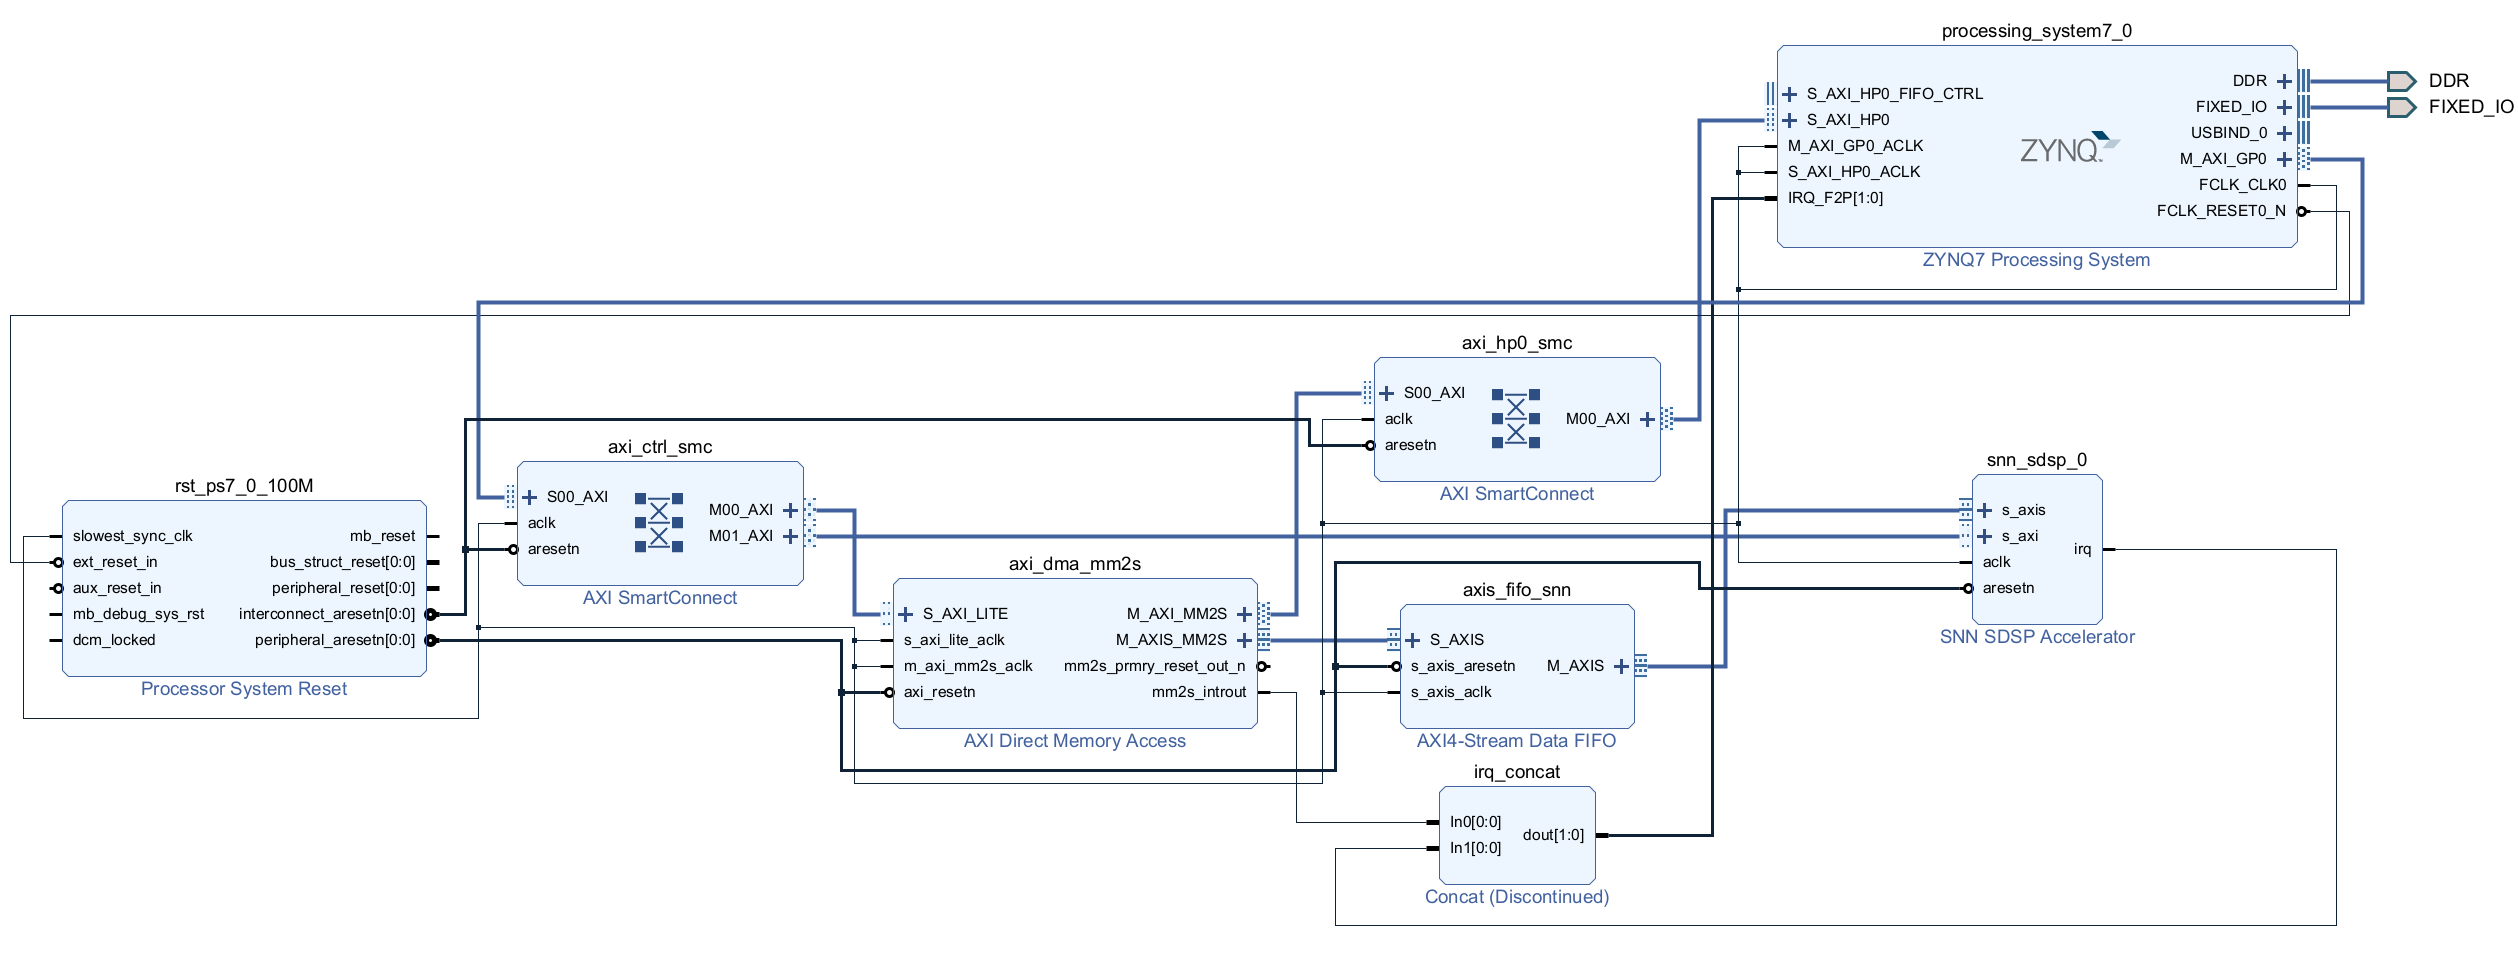
\includegraphics[width=1.06\linewidth]{figures/block_design.png}%
	}
	\caption{Final Vivado Block Design of the PYNQ-Z1 \gls{snn}-\gls{sdsp} System}
	\label{fig:final-block-design}
\end{figure}

\subsection{Control and Data-Movement Paths}

The design separates low-bandwidth control transactions from the bulk input-data transfer. The \gls{ps} accesses the programmable logic through its \texttt{M\_AXI\_GP0} master port. The control SmartConnect, \texttt{axi\_ctrl\_smc}, decodes this address space and provides two subordinate paths: one to the AXI-Lite control port of \texttt{axi\_dma\_mm2s} and one to the AXI-Lite slave port of \texttt{snn\_sdsp\_0}. Software can consequently configure the DMA and the accelerator independently through memory-mapped accesses.

Input spike trains are prepared in external DDR memory. The AXI DMA is configured in simple, memory-to-stream mode; its stream-to-memory channel and scatter-gather engine are not included because the accelerator returns its classification result and status through AXI-Lite rather than through an output stream. On the memory side, the DMA uses a 64-bit AXI master interface. Its read requests reach DDR through \texttt{axi\_hp0\_smc} and the high-performance \texttt{S\_AXI\_HP0} port of the processing system. On the stream side, the DMA emits 32-bit words containing \texttt{TKEEP} and \texttt{TLAST}, matching the input interface of the packaged accelerator.

An AXI4-Stream Data FIFO is inserted between the DMA and \texttt{snn\_sdsp\_0}. The FIFO stores up to 512 stream words and propagates both \texttt{TKEEP} and \texttt{TLAST}. Its purpose is to decouple burst-oriented DDR transfers from the accelerator's input backpressure. The DMA can therefore continue filling the FIFO while the two internal spike-vector buffers are temporarily occupied, provided that sufficient FIFO capacity remains. The FIFO does not alter the word order or packet boundary; reconstruction and validation of the 784-bit input vectors remain the responsibility of \texttt{snn\_axi\_wrapper}, as described in Section \ref{subsec:rtl-architecture}.

Table \ref{tab:block-design-address-map} summarizes the address assignments generated for the final block design. The two 64-KiB control regions are visible to the processing system through \texttt{M\_AXI\_GP0}. The DMA can read the lower 512 MiB of the processing-system memory map through the HP0 data path. Keeping control and data movement on separate AXI paths prevents the repeated spike-data reads from sharing the low-bandwidth register path used for configuration and result access.

\begin{table}[htbp]
	\centering
	\caption{Address Map of the Final Vivado Block Design}
	\label{tab:block-design-address-map}
	\small
	\begin{tabularx}{\linewidth}{@{}l l l X@{}}
		\toprule
		\textbf{Access path} & \textbf{Base address} & \textbf{Span} & \textbf{Purpose} \\
		\midrule
		PS GP0 to DMA & \texttt{0x4040\_0000} & 64 KiB & Configuration and status of the MM2S DMA channel \\
		PS GP0 to accelerator & \texttt{0x43C0\_0000} & 64 KiB & Accelerator control, learning configuration, status, spike counts, and classification result \\
		DMA to PS HP0 & \texttt{0x0000\_0000} & 512 MiB & Reading the input spike buffer from external DDR memory \\
		\bottomrule
	\end{tabularx}
\end{table}

\subsection{Clock and Reset Distribution}

The processing system generates \texttt{FCLK\_CLK0} at 100\,MHz. This clock drives the GP0 and HP0 AXI interfaces, both SmartConnect instances, the memory-mapped and streaming sides of the DMA, the stream FIFO, and the packaged accelerator. Using a common clock for the complete programmable-logic data path avoids additional clock-domain-crossing logic and keeps the AXI handshakes aligned with the internal network schedule.

The active-low \texttt{FCLK\_RESET0\_N} signal enters the Processor System Reset IP shown in Figure \ref{fig:final-block-design}. This block synchronizes reset release to the fabric clock and produces separate active-low reset nets for the interconnect and peripheral groups. The interconnect reset is connected to the two SmartConnect blocks, while the peripheral reset initializes the DMA, stream FIFO, and accelerator IP. This arrangement ensures that no AXI endpoint begins a transaction before its associated interconnect has left reset. The accelerator's software-triggered reset remains internal to \texttt{snn\_axi\_wrapper}; it clears the network and transaction state without resetting the surrounding DMA or AXI fabric.

\subsection{Interrupt Integration and Runtime Sequence}

Two programmable-logic interrupts are returned to the processing system. The DMA's \texttt{mm2s\_introut} signal is connected to input 0 of \texttt{irq\_concat}, and the accelerator interrupt is connected to input 1. The resulting two-bit vector drives \texttt{IRQ\_F2P[1:0]}. Keeping the two sources separate allows processor-side software to distinguish completion or error events generated by the DMA from completion of the neural-network transaction. Within the accelerator, the interrupt is asserted when the classification result has been committed and the interrupt-enable control bit is set. It remains asserted through the sticky completion state until software clears that state.

At runtime, the processor first loads the overlay and places the packed input spike sequence in a contiguous DDR buffer. It then programs the learning enable, teacher enable, target label, teacher current, and learning-event intervals through the accelerator's AXI-Lite register space, configures the MM2S transfer, and issues the accelerator start command. The DMA reads the buffer through HP0 and streams the words through the FIFO into the packaged IP. After all configured time steps have been accepted and processed, the accelerator completes its sequential output scan, stores the winning class and individual spike counts, and raises its interrupt when enabled. The processor can then read the result through AXI-Lite without requiring a return DMA channel. This transaction sequence confines high-volume movement to the DDR-to-stream path and retains deterministic online learning entirely inside the programmable logic.

\section{PYNQ Runtime Control and Data Preparation}
\label{subsec:pynq-runtime-control}

The processor-side runtime provides the operational boundary between an experiment and the hardware system described in Section \ref{subsec:block-design-integration}. Its responsibilities are limited to loading the overlay, preparing the spike representation expected by the AXI wrapper, configuring one accelerator transaction, and retrieving its results. Membrane integration and synaptic-weight updates are not reproduced in software. Consequently, the processor remains outside the time-critical learning loop and the behaviour of \gls{sdsp} is determined by the programmable-logic implementation.

Figure \ref{fig:pynq-runtime-workflow} summarizes the resulting workflow. Control and status use AXI4-Lite, whereas the substantially larger spike sequence is transferred from DDR through the MM2S DMA path. This separation allows the same allocated input buffer and overlay instance to be reused across multiple samples while the software changes only the sample data and the run-specific control values.

\begin{figure}[t]
	\centering
	\makebox[\linewidth][c]{%
		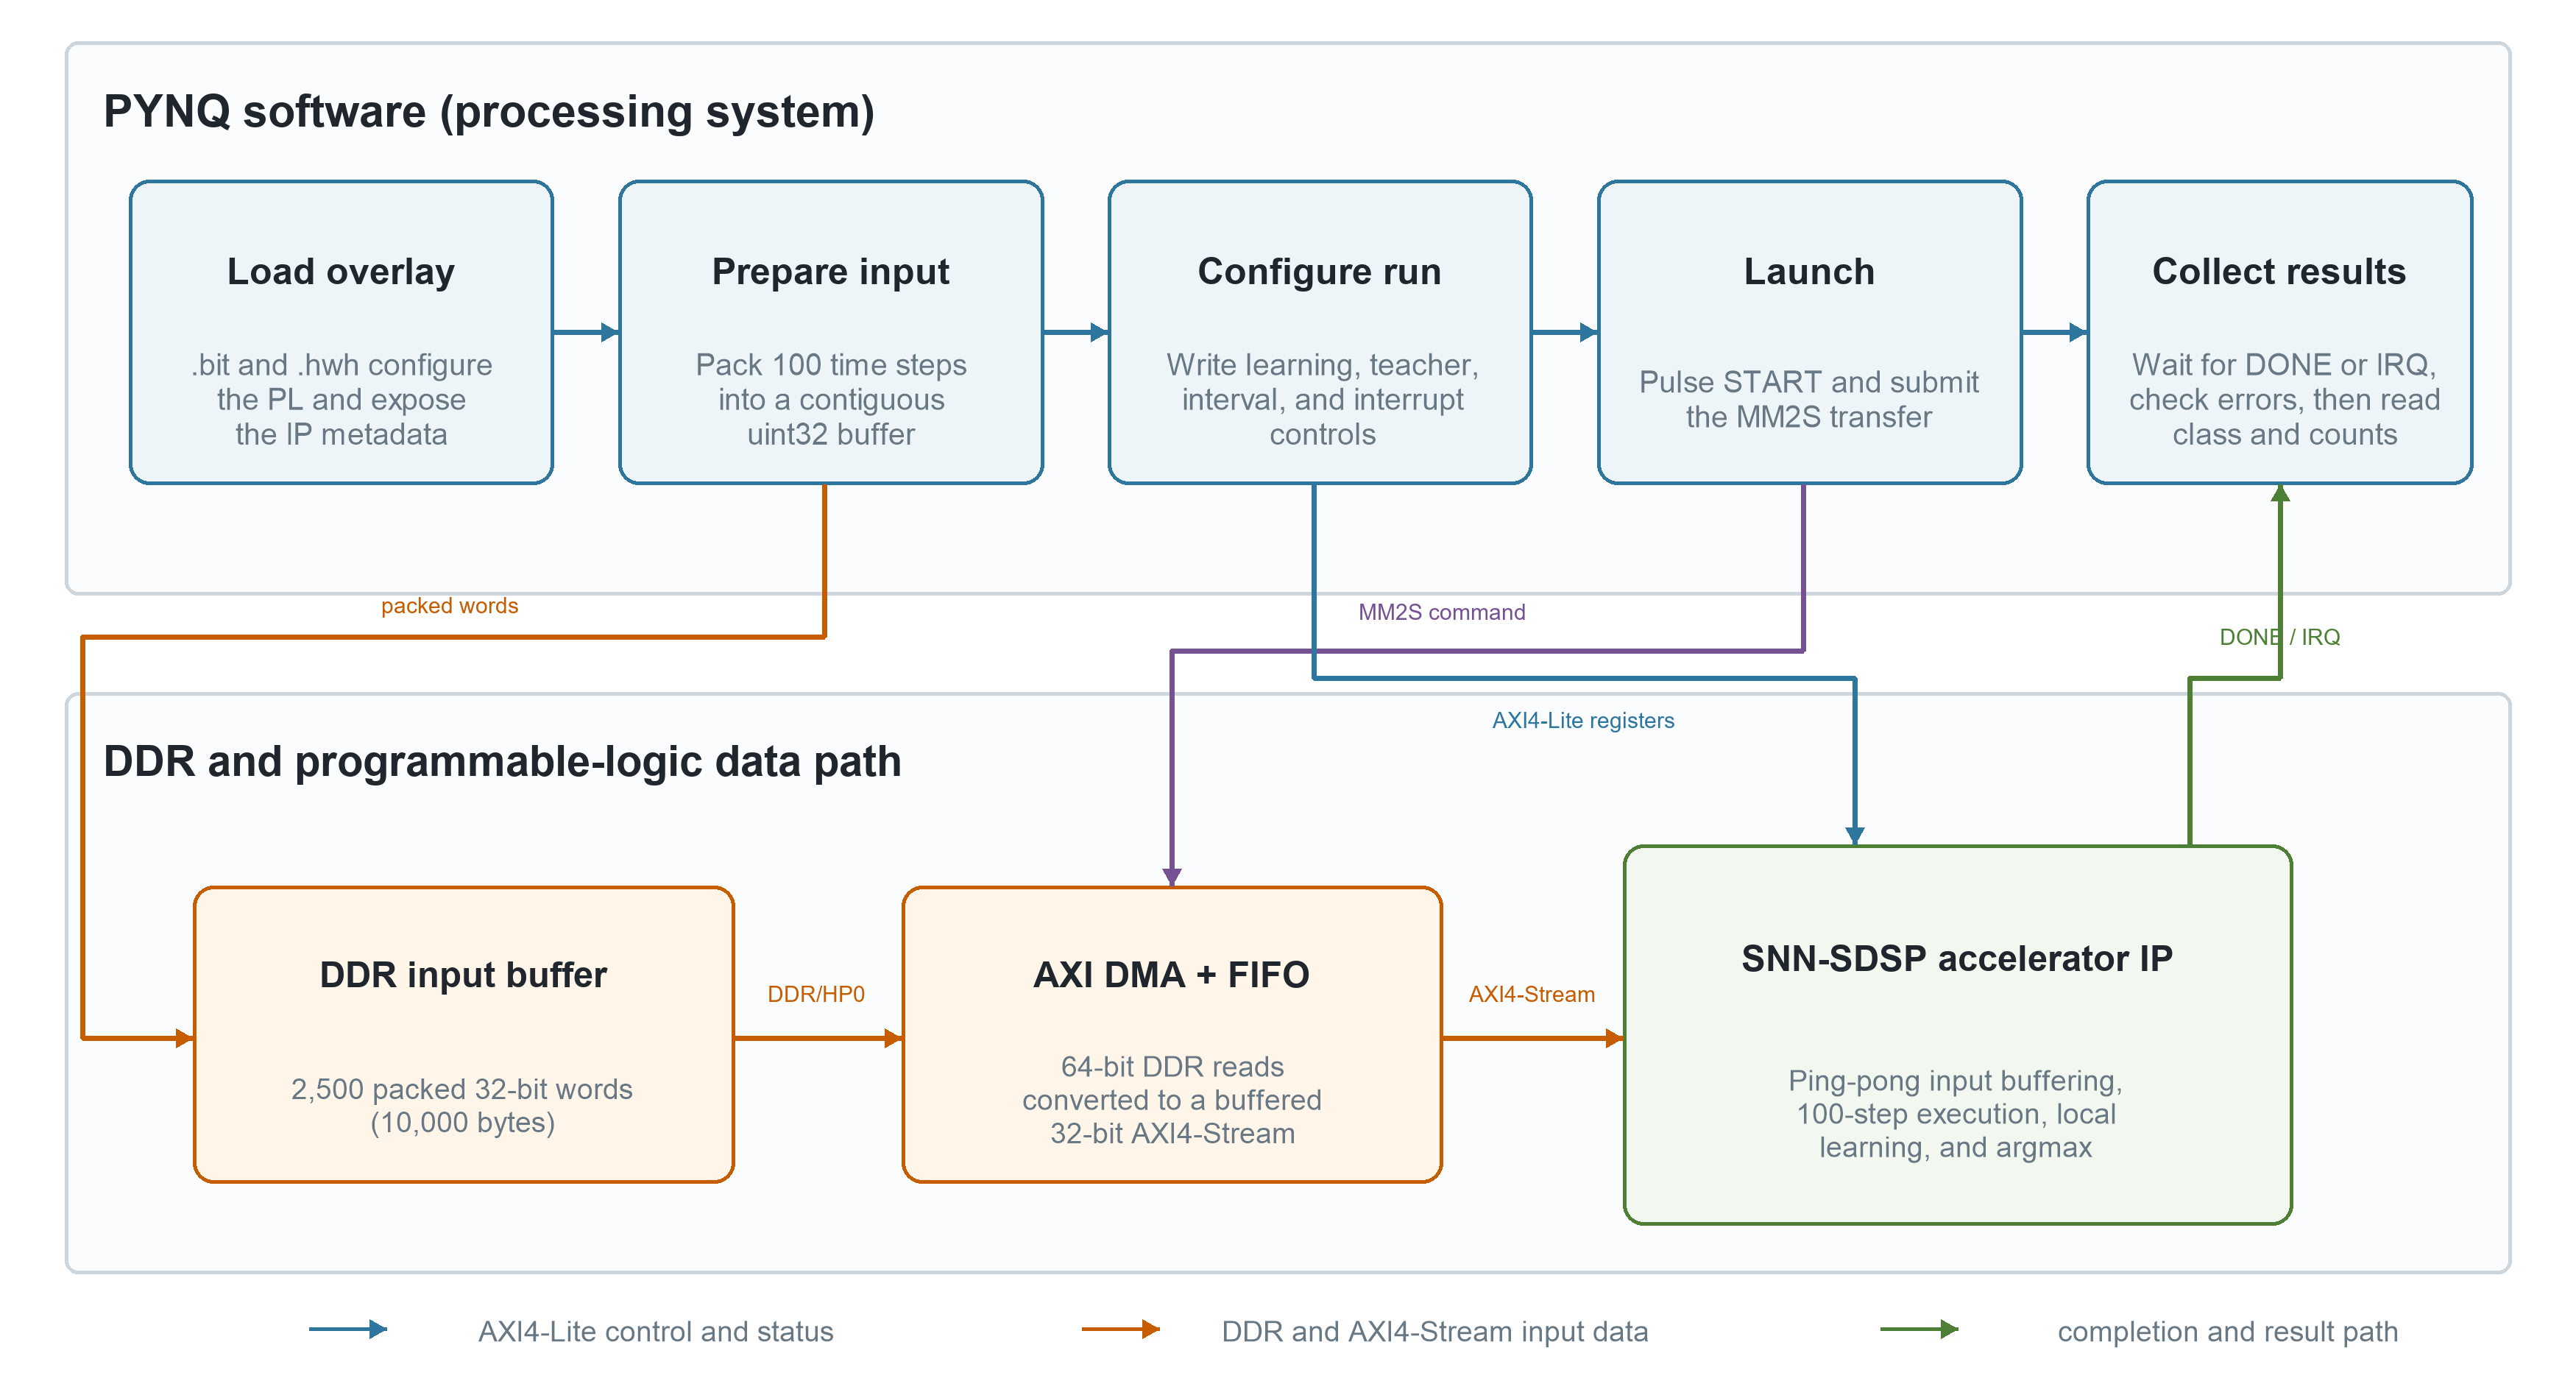
\includegraphics[width=1.06\linewidth]{figures/pynq_runtime_workflow.png}%
	}
	\caption{End-to-End PYNQ Runtime Workflow for One Accelerator Transaction}
	\label{fig:pynq-runtime-workflow}
\end{figure}

\subsection{Overlay Initialization and Register Interface}

The generated bitstream and hardware handoff file are deployed with the same overlay name. Loading the bitstream through the PYNQ \texttt{Overlay} class configures the programmable logic, while the \texttt{.hwh} metadata makes the DMA, accelerator address space, and interrupt connections visible to Python \cite{PYNQOverlayLoading}. The final design exposes the two relevant blocks as \texttt{axi\_dma\_mm2s} and \texttt{snn\_sdsp\_0}. A dedicated software driver is not required for the custom accelerator because its command and result registers can be accessed through the memory-mapped interface provided by the overlay.

Table \ref{tab:snn-axi-register-map} lists the implemented accelerator registers. The control register combines single-cycle commands with persistent mode bits. \texttt{START}, \texttt{SOFT\_RESET}, and \texttt{CLEAR\_DONE} are interpreted as command pulses, whereas the learning, bistability, interrupt, and teacher enables remain stored until software changes them. The target label, teacher current, and enable state are written before \texttt{START}; the teacher-related values are then captured for the complete transaction so that later processor writes cannot change supervision while a sample is being processed.

\begin{table}[htbp]
	\centering
	\caption{Software-Visible Register Map of \texttt{snn\_sdsp\_0}}
	\label{tab:snn-axi-register-map}
	\small
	\begin{tabularx}{\linewidth}{@{}l l X@{}}
		\toprule
		\textbf{Offset} & \textbf{Access} & \textbf{Function} \\
		\midrule
		\texttt{0x00} & R/W & Control: start, soft reset, learning enable, bistability enable, interrupt enable, completion clear, and teacher enable \\
		\texttt{0x04} & R & Status: idle, busy, completion, stream-format errors, active state, and input-buffer validity \\
		\texttt{0x08} & R & Number of time steps configured in the hardware instance \\
		\texttt{0x0C} & R/W & Four-bit target class used for teacher supervision \\
		\texttt{0x10} & R/W & Calcium-leak event interval \\
		\texttt{0x14} & R/W & Bistability event interval \\
		\texttt{0x18} & R/W & Teacher-current value applied to the selected output neuron \\
		\texttt{0x20} & R & Classification result produced by the final argmax scan \\
		\texttt{0x24--0x48} & R & Ten 32-bit output-neuron spike counters \\
		\texttt{0x50} & R & Number of input time steps accepted by the network \\
		\texttt{0x54} & R & Stream and execution progress, including word and completed-step counters \\
		\bottomrule
	\end{tabularx}
\end{table}

The status and progress registers also support debugging without introducing signals at the board boundary. In normal operation, software needs only the busy, completion, and error flags. The accepted-step and progress values are useful when distinguishing malformed input data from a stalled network transaction. A soft reset can clear the network and wrapper state without reconfiguring the complete overlay. It does not reload the initialized excitatory memory, so learned weights remain available for subsequent samples until the programmable logic is reconfigured.

\subsection{Spike Packing and DMA Transfer}

The input representation is prepared as an array of unsigned 32-bit words. Each 784-neuron time step occupies 25 words: the first 24 words carry 768 spike bits, and the lower 16 bits of the final word carry the remaining spikes. The unused upper half of the final word is set to zero. With the implemented value of 100 time steps, one accelerator transaction therefore contains 2,500 words, corresponding to 10,000 bytes. Software can read the configured time-step count from offset \texttt{0x08} instead of duplicating this value as a separate runtime constant.

The packed array is placed in a physically contiguous PYNQ buffer created with \texttt{pynq.allocate}, which provides the memory layout and device-visible address required by the DMA \cite{PYNQBuffer}. After the array has been populated, its contents are synchronized to the device when required by the selected memory configuration. The PYNQ DMA interface then submits the complete buffer to the MM2S channel \cite{PYNQDMA}. The transfer length defines the AXI4-Stream packet, causing \texttt{TLAST} to accompany only its final word. All transferred words contain four valid bytes, matching the \texttt{TKEEP=1111} check performed by \texttt{snn\_axi\_wrapper}.

No processor-side throttling is required between individual time steps. Backpressure from the accelerator propagates through the AXI4-Stream FIFO to the DMA, while the two internal input buffers allow transmission and neural processing to overlap. The software therefore submits one contiguous transaction rather than repeatedly controlling the DMA for each 784-bit vector. This both reduces processor involvement and preserves the packet boundary checked by the hardware.

\subsection{Transaction Completion and Result Retrieval}

Before starting a sample, software clears a previous completion flag and programs the desired operating mode. For inference, learning and teacher supervision are disabled. For online learning, software additionally writes the target label, teacher current, calcium-leak interval, and optional bistability configuration. These values must be valid before the \texttt{START} pulse because the supervision parameters are captured when the new transaction is accepted.

The start request may be issued before the first stream word arrives. In this case, the wrapper retains it as \texttt{start\_pending} and activates the network only after one complete time-step vector is available. Software can therefore launch the accelerator and the MM2S transfer without cycle-level coordination. During execution, the DMA and accelerator interrupts remain independent: the DMA interrupt indicates completion of the memory-to-stream transfer, whereas the accelerator interrupt indicates that all network outputs have been processed and the classification result is valid.

Completion can be detected either by waiting for the accelerator interrupt or by polling the completion bit at offset \texttt{0x04}. The stream and \texttt{TLAST} error flags are checked before the result is accepted. Software then reads the predicted class from offset \texttt{0x20} and, when detailed evaluation is required, the ten spike counters from offsets \texttt{0x24} to \texttt{0x48}. Finally, \texttt{CLEAR\_DONE} acknowledges the completed transaction. The same overlay and allocated buffer can then be reused for the next sample; only reloading the bitstream restores the original initialized synaptic weights.

\section{Verification Infrastructure and Test Strategy}
\label{subsec:verification-infrastructure}

Verification was organized as a sequence of increasingly integrated checks rather than as a single end-to-end simulation. This structure was necessary because an incorrect final classification can originate from several different sources, including the learning rule, the generated network schedule, AXI stream framing, or processor-side data preparation. Exercising these boundaries independently makes a failure observable close to its source and reduces the number of internal signals that must be inspected at the system level.

Figure \ref{fig:verification-strategy} shows the four verification levels used for the implementation. Module-level tests establish the behaviour of the learning primitives and writable memory. Layer and network tests then check the timing contracts inherited from Spiker+. AXI-wrapper tests verify the complete hardware transaction boundary, while the final level compares board-produced observations with a software reference using preserved input data. Quantitative results obtained with this infrastructure are reported in Chapter \ref{sec:results_and_evaluation}; this section describes only how the checks were constructed.

\begin{figure}[t]
	\centering
	\makebox[\linewidth][c]{%
		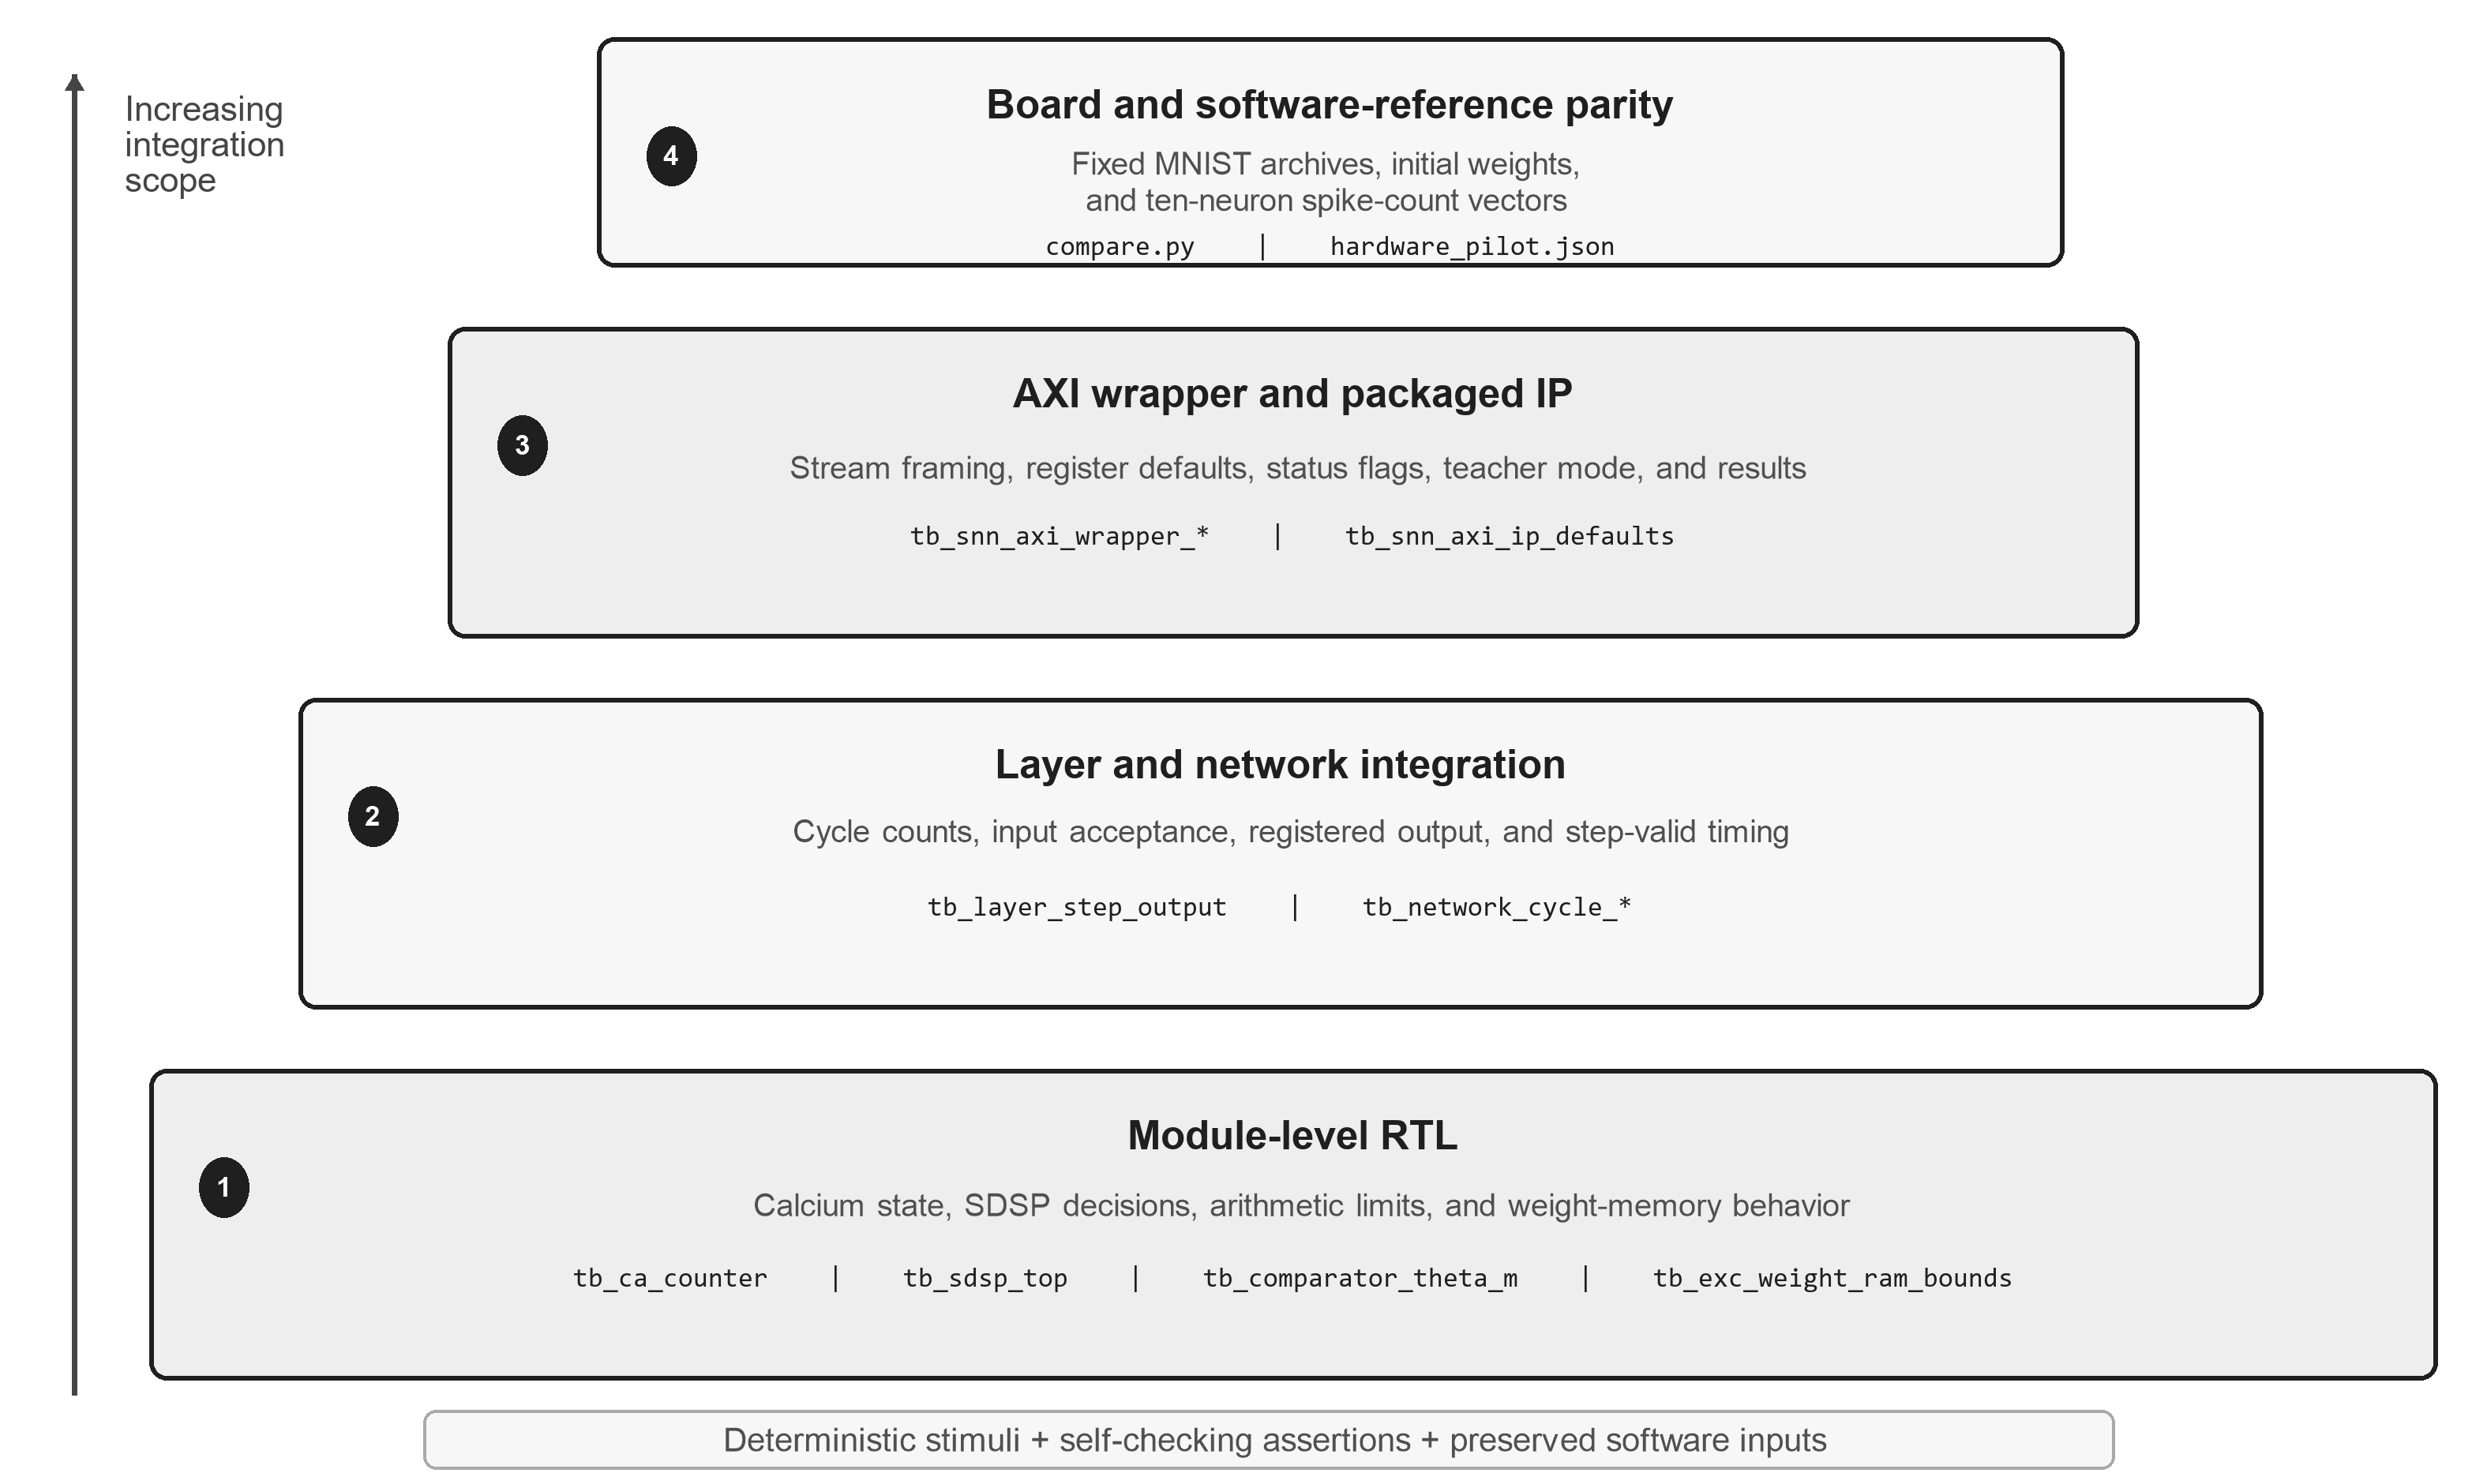
\includegraphics[width=1.04\linewidth]{figures/verification_strategy.png}%
	}
	\caption{Layered Verification Strategy for the Implemented System}
	\label{fig:verification-strategy}
\end{figure}

\subsection{Module-Level RTL Verification}

The lowest verification level uses self-checking VHDL testbenches for the individual \gls{sdsp} building blocks. The calcium counter tests exercise reset, increments caused by postsynaptic spikes, leak events, simultaneous spike-and-leak handling, and saturation at the representable limits. The condition comparator is tested around the signed membrane-potential threshold and the calcium boundaries, ensuring that the generated \texttt{up} and \texttt{down} conditions change at the intended encoded values. Separate tests cover the delta-weight generator, full-adder-based update path, overflow handling, and the integrated \texttt{sdsp\_top} unit.

The writable excitatory memory receives an additional boundary test because its address range is narrower than the ten-bit address signal. The testbench reads the first and final valid entries, checks that the unused prefetched address returns a defined zero value, and verifies read-first behaviour during a weight write. These checks directly target the last-address condition created by the Spiker+ prefetch schedule. A separate synthesis script checks that the 784-by-30-bit description is inferred as block memory; functional simulation alone cannot establish the selected FPGA storage primitive.

All unit tests use assertions rather than relying only on waveform inspection. A mismatch therefore terminates the simulation at the first violated property and identifies the expected interface contract. Waveforms remain useful for diagnosing a failure, but they are not the sole acceptance criterion.

\subsection{Network and AXI Integration Tests}

The second level verifies the interfaces between the generated controller, the modified layer, and the network wrapper. Cycle-count testbenches count the \texttt{sample}, \texttt{input\_accept}, and \texttt{out\_spikes\_valid} events and compare them with the configured number of time steps. The layer-output testbench separately checks that the output exported with \texttt{step\_valid} is the value already captured by the output barrier. This isolates the network schedule from AXI behaviour and verifies the transaction boundaries used by the ping-pong buffers.

At the wrapper level, AXI4-Stream stimuli reproduce the same 25-word representation used on the board. Short two-step tests provide rapid feedback for handshakes, word assembly, completion state, and result access. The full-size test transfers 2,500 words and checks the accepted- and completed-step counts for a 100-step transaction. Its selectable stimulus modes cover the normal sparse stream, dense input activity, zero-input control behaviour, and teacher-enabled zero-input operation. The dense case makes the output path observable, while the paired teacher-enabled and teacher-disabled cases isolate the contribution of the supervision current.

AXI-Lite accesses are generated by reusable write and read procedures inside the testbenches. They configure the same registers used by PYNQ software and subsequently inspect status, progress, classification, and spike-count values. An additional packaged-IP test verifies that customization defaults appear after hardware reset, that processor writes override them, and that reset restores the configured defaults. Table \ref{tab:verification-artifacts} summarizes the representative verification artifacts and their primary checks. Together, these tests cover both the internal computation schedule and the software-visible contract of \texttt{snn\_sdsp\_0}.

\begin{table}[htbp]
	\centering
	\caption{Representative Verification Artifacts and Their Primary Checks}
	\label{tab:verification-artifacts}
	\small
	\begin{tabularx}{\linewidth}{@{}p{0.20\linewidth}p{0.34\linewidth}X@{}}
		\toprule
		\textbf{Scope} & \textbf{Representative artifact} & \textbf{Primary check} \\
		\midrule
		SDSP modules & \texttt{tb\_ca\_counter}, \texttt{tb\_sdsp\_top} & State transitions, update selection, saturation, and event handling \\
		Comparator and RAM & \texttt{tb\_comparator\_theta\_m}, \texttt{tb\_exc\_weight\_ram\_bounds} & Signed threshold boundary, valid address range, read-first semantics, and write-back \\
		Layer and network & \texttt{tb\_layer\_step\_output}, \texttt{tb\_network\_cycle\_count} & Registered output alignment and agreement between requested, accepted, and completed steps \\
		AXI wrapper & \texttt{tb\_snn\_axi\_wrapper\_two\_steps}, \texttt{tb\_snn\_axi\_wrapper\_100\_steps} & Stream handshakes, packet assembly, modes, status, results, and completion \\
		Packaged IP & \texttt{tb\_snn\_axi\_ip\_defaults} & IP customization defaults, AXI register overrides, and reset restoration \\
		Cross-domain comparison & \texttt{compare.py} & Input identity, initial-weight decoding, and per-neuron spike-count comparison \\
		\bottomrule
	\end{tabularx}
\end{table}

\subsection{Hardware--Software Parity and Reproducibility}

The highest verification level compares observations from the deployed design with the Spiker+ software model. The comparison uses stored spike archives rather than regenerating stochastic spike trains for each run. Each archive records the packed words, labels, time-step count, gain, and bit order, while a SHA-256 digest identifies the exact training input used by the board experiment. Preserving the input realization is essential because two independently generated stochastic encodings of the same image do not provide a sample-by-sample comparison.

The comparison script decodes the VHDL initialization package into the same ten-by-784 weight matrix used by the software model. It first checks the weight-code distribution and verifies whether the software and hardware initial states are identical. It then applies the preserved input words to the software model and compares the ten output-neuron spike counts with the board observations. Comparing the complete count vector is more informative than comparing only the winning class, since different internal behaviour can still produce the same argmax result.

This parity step is intentionally treated as a diagnostic comparison rather than as proof of cycle-accurate equivalence. The software model uses floating-point neuron dynamics, whereas the implemented datapath uses fixed-point arithmetic and an explicit multi-cycle schedule. Any remaining difference must therefore be interpreted together with the lower verification levels. The script prevents a training comparison from being presented as exact parity unless the initial-state and baseline conditions have first been established; an explicitly forced run is labelled only as a trend comparison.

Board observations are stored separately from the comparison script, and the script does not reprogram the device or modify the preserved data. This separation makes the experiment repeatable and prevents a software rerun from silently changing the hardware stimulus. The same fixed evaluation archive can consequently be used before and after online learning, allowing changes in the output distribution to be attributed to the learned synaptic state rather than to a different stochastic input realization.

\section{Chapter Summary}
\label{subsec:implementation-summary}

This chapter presented the implementation of the proposed online-learning \gls{snn} on the PYNQ-Z1 platform. The Spiker+-generated network, the modified neuron and synaptic-memory modules, and the \gls{sdsp} learning logic were integrated beneath \texttt{snn\_axi\_wrapper} and packaged as a reusable Vivado \gls{ip} core. The final block design connects this accelerator to the Zynq processing system through an AXI4-Lite control path, an AXI DMA and stream FIFO for spike-data transfer, a shared clock and reset structure, and separate DMA and accelerator interrupts.

On the processor side, the PYNQ overlay and runtime interface provide input preparation, register configuration, transaction control, and result retrieval, while spike processing and synaptic updates remain inside the programmable logic. A layered verification environment was established from self-checking module simulations through network and AXI integration tests to board-level comparison with preserved software inputs. Together, these implementation and verification components provide the deployable system used for the functional, resource, timing, and learning evaluations presented in Chapter \ref{sec:results_and_evaluation}.
